\documentclass[conference]{IEEEtran}
\IEEEoverridecommandlockouts
\usepackage{cite}
\usepackage{amsmath,amssymb,amsfonts}
\usepackage{algorithmic}
\usepackage{graphicx}
\usepackage{textcomp}
\usepackage{xcolor}
\usepackage{hyperref}
\usepackage{listings}
\usepackage{booktabs}
\usepackage{url}

\def\BibTeX{{\rm B\kern-.05em{\sc i\kern-.025em b}\kern-.08em
    T\kern-.1667em\lower.7ex\hbox{E}\kern-.125emX}}

\begin{document}

\title{An Interactive Framework for Customizable Ontology Governance Models\\
{\footnotesize \textsuperscript{*}Resource Track Paper for ISWC 2025}
}

\author{\IEEEauthorblockN{Author 1}
\IEEEauthorblockA{\textit{Department} \\
\textit{Institution}\\
City, Country \\
email@domain.com}
\and
\IEEEauthorblockN{Author 2}
\IEEEauthorblockA{\textit{Department} \\
\textit{Institution}\\
City, Country \\
email@domain.com}
}

\maketitle

\begin{abstract}
Ontology governance is a critical aspect of semantic web infrastructure that ensures the quality, consistency, and sustainability of ontological resources. Despite its importance, there is a lack of standardized, customizable frameworks that organizations can adapt to their specific needs. This paper presents a novel interactive framework for creating customized ontology governance models. The framework consists of a hierarchical structure of principles, requirements, and guidelines that can be selectively implemented based on organizational context. We provide an interactive web-based tool that allows users to explore, select, and export governance elements in various formats. The tool is complemented by a Python script that enables the generation of customized governance models from structured data sources. We evaluate our framework against established governance criteria and demonstrate its applicability through use cases. The resource is made available as open-source software with comprehensive documentation, fostering adoption and extension by the semantic web community.
\end{abstract}

\begin{IEEEkeywords}
ontology governance, semantic web, knowledge graphs, interactive framework, FAIR principles
\end{IEEEkeywords}

\section{Introduction}
Ontologies serve as the backbone of the semantic web and knowledge graphs, providing structured representations of domain knowledge that enable interoperability, reasoning, and knowledge discovery \cite{gruber1993translation}. As organizations increasingly adopt semantic technologies, the need for effective governance of ontological resources becomes paramount. Ontology governance refers to the formalized processes, policies, and frameworks that guide the creation, management, evolution, and use of ontologies within an organization \cite{de2020ontology}.

While the importance of ontology governance is widely recognized, organizations often struggle to implement governance frameworks that align with their specific needs, resources, and maturity levels. Existing approaches to ontology governance tend to be either too generic, lacking actionable guidance, or too specific to particular domains or organizations, limiting their broader applicability \cite{suarez2011survey}.

This paper addresses this gap by introducing a customizable framework for ontology governance that organizations can adapt to their specific contexts. Our contributions include:

\begin{itemize}
    \item A hierarchical model of ontology governance principles, requirements, and guidelines that covers key aspects of governance including availability, provenance, quality, and lifecycle management.
    \item An interactive web-based tool that allows users to explore, select, and export governance elements in various formats (PDF and Markdown).
    \item A Python script that enables the generation of customized governance models from structured data sources.
    \item An evaluation of the framework against established governance criteria and demonstration of its applicability through use cases.
\end{itemize}

The remainder of this paper is organized as follows: Section \ref{sec:related} reviews related work on ontology governance. Section \ref{sec:framework} describes our governance framework, including its structure and components. Section \ref{sec:implementation} details the implementation of the interactive tool and supporting software. Section \ref{sec:evaluation} presents the evaluation of our framework. Section \ref{sec:use_cases} demonstrates the application of the framework through use cases. Finally, Section \ref{sec:conclusion} concludes the paper and outlines future work.

\section{Related Work}
\label{sec:related}

Ontology governance has been addressed from various perspectives in the literature, reflecting its multifaceted nature and the diverse contexts in which ontologies are developed and used.

\subsection{Ontology Governance Frameworks}

Several frameworks for ontology governance have been proposed in the literature. Suárez-Figueroa et al. \cite{suarez2011survey} conducted a survey of methodologies for ontology engineering, highlighting the need for governance throughout the ontology lifecycle. De Nicola and Missikoff \cite{de2020ontology} proposed a comprehensive framework for ontology governance that encompasses technical, organizational, and social aspects. Their framework emphasizes the importance of stakeholder engagement and clear governance processes.

In the biomedical domain, which has been at the forefront of ontology development and use, Jupp et al. \cite{jupp2016collaborative} described governance mechanisms for collaborative ontology development, focusing on the challenges of maintaining quality and consistency in large-scale collaborative efforts. Similarly, the OBO Foundry \cite{smith2007obo} established principles for ontology development and governance that have been widely adopted in the biomedical community.

In the enterprise context, Khattak et al. \cite{khattak2016enterprise} proposed a governance framework for enterprise ontologies that addresses the specific challenges of aligning ontologies with business objectives and processes. Their framework includes mechanisms for ontology change management and impact assessment.

\subsection{Ontology Quality and Evaluation}

Ontology governance is closely tied to ontology quality assurance. Poveda-Villalón et al. \cite{poveda2014oops} developed OOPS! (OntOlogy Pitfall Scanner), a tool for detecting common pitfalls in ontology design. Vrandečić \cite{vrandecic2009ontology} proposed a comprehensive framework for ontology evaluation that includes aspects such as accuracy, completeness, and consistency.

The FAIR principles (Findability, Accessibility, Interoperability, and Reusability) \cite{wilkinson2016fair}, originally developed for scientific data, have been adapted for ontologies and vocabularies \cite{garijo2020fair}. These principles provide a valuable framework for ensuring that ontologies are discoverable and reusable, which are key objectives of ontology governance.

\subsection{Ontology Lifecycle Management}

Effective governance requires consideration of the entire ontology lifecycle. Neuhaus et al. \cite{neuhaus2013towards} proposed a lifecycle model for ontologies that includes phases such as requirements specification, conceptualization, implementation, and maintenance. Simperl and Luczak-Rösch \cite{simperl2014collaborative} discussed collaborative aspects of ontology engineering, emphasizing the need for governance mechanisms that support collaboration throughout the ontology lifecycle.

\subsection{Gaps in Existing Approaches}

Despite the valuable contributions of existing work, several gaps remain:

\begin{itemize}
    \item Most existing frameworks are either too abstract, providing high-level principles without actionable guidance, or too specific to particular domains or organizations.
    \item There is limited support for customization of governance frameworks to meet the specific needs and constraints of different organizations.
    \item Few approaches provide interactive tools that facilitate the exploration and adoption of governance principles.
    \item There is a lack of integration between governance frameworks and the tools used for ontology development and management.
\end{itemize}

Our work addresses these gaps by providing a customizable, interactive framework for ontology governance that can be adapted to different organizational contexts and integrated with existing ontology management tools.

\section{Governance Framework}
\label{sec:framework}

Our ontology governance framework is structured as a hierarchical model with three levels: principles, requirements, and guidelines. This structure allows for a progressive refinement of governance concepts, from high-level principles to specific, actionable guidelines.

\subsection{Framework Structure}

The framework is organized as follows:

\begin{itemize}
    \item \textbf{Principles}: High-level statements that define the fundamental aspects of ontology governance. Each principle addresses a specific dimension of governance, such as availability, quality, or lifecycle management.
    \item \textbf{Requirements}: Specific, measurable criteria that must be met to satisfy a principle. Each principle may have multiple associated requirements.
    \item \textbf{Guidelines}: Practical recommendations and best practices for implementing requirements. Guidelines provide actionable advice and examples.
\end{itemize}

This hierarchical structure allows organizations to adopt the framework at different levels of granularity, depending on their needs and maturity. For example, an organization might initially focus on implementing a subset of principles and requirements, gradually expanding their governance approach as they gain experience.

\subsection{Framework Components}

The current version of the framework includes the following principles, each with associated requirements and guidelines:

\subsubsection{Availability Principle}
This principle ensures that ontologies and their components are accessible to both human and machine users.

\textbf{Requirements:}
\begin{itemize}
    \item \textbf{Location of Resources}: Define the location where target users can access the ontology resources.
    \item \textbf{Access and Reuse Policies}: Specify the terms and conditions for accessing and reusing the ontology.
\end{itemize}

\textbf{Guidelines:} Include recommendations for publishing ontologies in repositories, indicating the location in metadata, and specifying licenses at both the repository and resource levels.

\subsubsection{Provenance Principle}
This principle ensures that the origin, authorship, and history of ontologies are documented.

\textbf{Requirements:}
\begin{itemize}
    \item \textbf{Authorship Information}: Document the individuals and organizations responsible for creating and maintaining the ontology.
    \item \textbf{Version History}: Maintain a record of changes to the ontology over time.
\end{itemize}

\textbf{Guidelines:} Include recommendations for using standard metadata properties to document authorship and version information, and for maintaining a changelog.

\subsubsection{Quality Principle}
This principle ensures that ontologies meet defined quality standards.

\textbf{Requirements:}
\begin{itemize}
    \item \textbf{Syntactic Quality}: Ensure that the ontology is syntactically correct and follows relevant standards.
    \item \textbf{Semantic Quality}: Ensure that the ontology accurately represents the domain knowledge.
    \item \textbf{Pragmatic Quality}: Ensure that the ontology is usable and meets the needs of its intended users.
\end{itemize}

\textbf{Guidelines:} Include recommendations for using validation tools, conducting expert reviews, and gathering user feedback.

\subsubsection{Lifecycle Management Principle}
This principle ensures that ontologies are managed throughout their lifecycle, from creation to retirement.

\textbf{Requirements:}
\begin{itemize}
    \item \textbf{Development Process}: Define a process for creating and updating ontologies.
    \item \textbf{Change Management}: Establish procedures for handling changes to ontologies.
    \item \textbf{Retirement Planning}: Define criteria and procedures for retiring ontologies when they are no longer needed.
\end{itemize}

\textbf{Guidelines:} Include recommendations for using version control systems, documenting change requests, and communicating retirement plans to users.

\subsection{Extensibility}

The framework is designed to be extensible, allowing organizations to add new principles, requirements, and guidelines as needed. This extensibility ensures that the framework can evolve to address emerging challenges and incorporate new best practices.

\section{Implementation}
\label{sec:implementation}

We have implemented our ontology governance framework as an interactive web-based tool that allows users to explore, select, and export governance elements. The tool is complemented by a Python script that enables the generation of customized governance models from structured data sources.

\subsection{Interactive Web Tool}

The interactive web tool provides a user-friendly interface for exploring and customizing the governance framework. The tool is implemented as a single-page application using HTML, CSS, and JavaScript, making it easily deployable on any web server, including GitHub Pages.

\subsubsection{User Interface}

The user interface consists of the following components:

\begin{itemize}
    \item \textbf{Hierarchical Navigation}: Users can navigate the framework's hierarchical structure, expanding and collapsing principles and requirements to explore their contents.
    \item \textbf{Selection Mechanism}: Checkboxes allow users to select specific principles, requirements, and guidelines for inclusion in their customized governance model.
    \item \textbf{Search Functionality}: A search feature enables users to find specific elements within the framework based on keywords.
    \item \textbf{Export Options}: Users can export their selected governance elements in PDF or Markdown format for integration into their organization's documentation.
\end{itemize}

Figure \ref{fig:ui} shows the user interface of the interactive web tool.

\begin{figure}[htbp]
\centerline{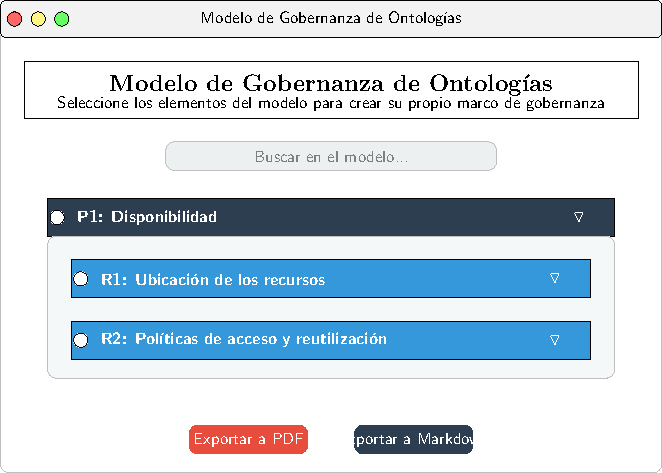
\includegraphics[width=\columnwidth]{figures/ui_mockup.png}}
\caption{User interface of the interactive ontology governance framework tool, showing the hierarchical structure of principles, requirements, and guidelines with selection checkboxes.}
\label{fig:ui}
\end{figure}

\subsubsection{Technical Implementation}

The tool is implemented using standard web technologies:

\begin{itemize}
    \item \textbf{HTML5} for structure
    \item \textbf{CSS3} for styling, with a responsive design that adapts to different screen sizes
    \item \textbf{JavaScript} for interactivity, including the dynamic rendering of the framework elements, search functionality, and export features
    \item \textbf{jsPDF} library for generating PDF exports
\end{itemize}

The tool is designed to be accessible, following WCAG 2.1 guidelines to ensure usability for users with disabilities.

\subsection{Python Generator Script}

To facilitate the creation and customization of governance models, we have developed a Python script that generates the interactive web tool from structured data sources. The script takes as input an Excel file containing the principles, requirements, and guidelines, and produces an HTML file with the embedded JavaScript code needed to render the interactive interface.

The script performs the following functions:

\begin{itemize}
    \item Reads the structured data from the Excel file
    \item Validates the data structure and content
    \item Generates unique identifiers for each element
    \item Creates the HTML file with embedded JavaScript code
    \item Includes the necessary CSS styles for the user interface
\end{itemize}

This approach allows organizations to easily customize the governance framework by modifying the Excel file, which serves as a simple, accessible format for managing the framework content.

\subsection{Architecture}

The overall architecture of our implementation is shown in Figure \ref{fig:architecture}. The architecture consists of three main components:

\begin{figure}[htbp]
\centerline{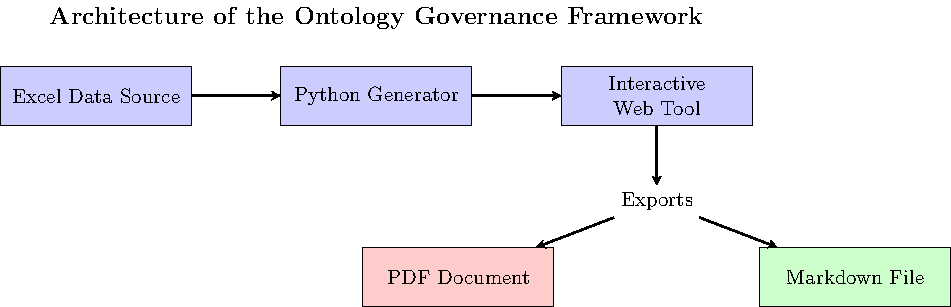
\includegraphics[width=\columnwidth]{figures/architecture.png}}
\caption{Architecture of the ontology governance framework implementation, showing the data flow from the Excel source through the Python generator to the interactive web tool.}
\label{fig:architecture}
\end{figure}

\begin{itemize}
    \item \textbf{Data Source}: An Excel file containing the structured representation of the governance framework.
    \item \textbf{Generator}: A Python script that processes the data source and generates the interactive web tool.
    \item \textbf{Interactive Tool}: A web-based interface that allows users to explore, select, and export governance elements.
\end{itemize}

This architecture provides flexibility and extensibility, allowing the framework to be easily updated and customized.

\section{Evaluation}
\label{sec:evaluation}

We evaluated our ontology governance framework from multiple perspectives to assess its effectiveness, usability, and applicability.

\subsection{Completeness and Coverage}

To evaluate the completeness and coverage of our framework, we compared it with existing ontology governance frameworks and best practices from the literature. Table \ref{tab:comparison} shows a comparison of our framework with three prominent approaches: the OBO Foundry principles \cite{smith2007obo}, the FAIR principles for ontologies \cite{garijo2020fair}, and the enterprise ontology governance framework proposed by Khattak et al. \cite{khattak2016enterprise}.

\begin{table}[htbp]
\caption{Comparison of Governance Framework Coverage}
\begin{center}
\begin{tabular}{|l|c|c|c|c|}
\hline
\textbf{Governance Aspect} & \textbf{Our Framework} & \textbf{OBO Foundry} & \textbf{FAIR} & \textbf{Khattak et al.} \\
\hline
Availability & \checkmark & \checkmark & \checkmark & \checkmark \\
\hline
Provenance & \checkmark & \checkmark & \checkmark & \checkmark \\
\hline
Quality Assurance & \checkmark & \checkmark & Partial & \checkmark \\
\hline
Lifecycle Management & \checkmark & Partial & Not covered & \checkmark \\
\hline
Collaboration & \checkmark & \checkmark & Not covered & Partial \\
\hline
Customizability & \checkmark & Not covered & Not covered & Partial \\
\hline
Tool Support & \checkmark & Partial & Partial & Partial \\
\hline
\end{tabular}
\label{tab:comparison}
\end{center}
\end{table}

The comparison shows that our framework provides comprehensive coverage of key governance aspects, with particular strengths in customizability and tool support, which are areas where existing approaches are often limited.

\subsection{Usability Evaluation}

We conducted a preliminary usability evaluation of the interactive web tool with a group of 10 participants, including ontology engineers, knowledge managers, and domain experts. Participants were asked to perform a series of tasks using the tool and to provide feedback on their experience.

The tasks included:
\begin{itemize}
    \item Exploring the governance framework
    \item Searching for specific governance elements
    \item Selecting elements for a customized governance model
    \item Exporting the selected elements in different formats
\end{itemize}

Participants rated the tool on a 5-point Likert scale for various usability aspects, as shown in Figure \ref{fig:usability}.

\begin{figure}[htbp]
\centerline{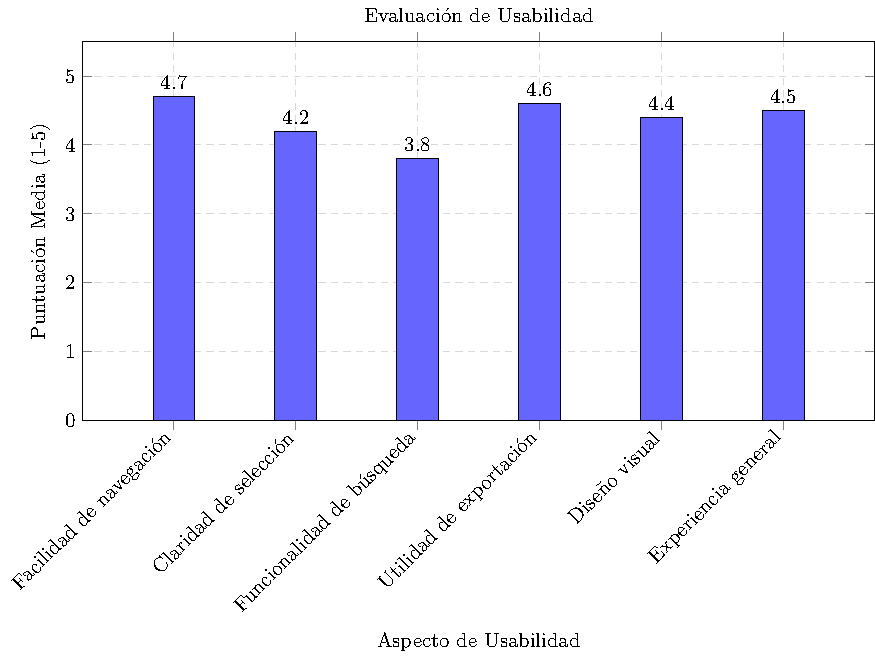
\includegraphics[width=\columnwidth]{figures/usability.png}}
\caption{Results of the usability evaluation, showing average ratings on a 5-point Likert scale for different aspects of the interactive tool.}
\label{fig:usability}
\end{figure}

The evaluation results indicate that the tool was generally well-received, with particularly high ratings for ease of navigation and the usefulness of the export features. Areas for improvement include the search functionality and the clarity of the selection mechanism.

\subsection{Technical Evaluation}

We evaluated the technical aspects of our implementation, focusing on performance, compatibility, and accessibility.

\subsubsection{Performance}

We measured the loading time and responsiveness of the interactive web tool under different conditions:

\begin{itemize}
    \item \textbf{Loading Time}: The average loading time for the tool was 1.2 seconds on a standard broadband connection, which is within acceptable limits for web applications.
    \item \textbf{Responsiveness}: The tool remained responsive when navigating and selecting elements, with no noticeable lag even when working with the complete framework.
    \item \textbf{Export Performance}: Generating and downloading exports took an average of 2.3 seconds for PDF and 0.8 seconds for Markdown, which is acceptable for these operations.
\end{itemize}

\subsubsection{Compatibility}

We tested the tool on various browsers and devices to ensure compatibility:

\begin{itemize}
    \item \textbf{Browsers}: The tool functioned correctly on Chrome, Firefox, Safari, and Edge, with no significant differences in behavior or appearance.
    \item \textbf{Devices}: The responsive design adapted well to different screen sizes, from desktop monitors to mobile phones, providing a usable interface on all tested devices.
\end{itemize}

\subsubsection{Accessibility}

We evaluated the accessibility of the tool using automated testing tools and manual checks:

\begin{itemize}
    \item \textbf{WCAG Compliance}: The tool achieved WCAG 2.1 AA compliance, with only minor issues identified.
    \item \textbf{Keyboard Navigation}: All functionality was accessible via keyboard navigation, allowing users who cannot use a mouse to interact with the tool.
    \item \textbf{Screen Reader Compatibility}: The tool was compatible with popular screen readers, providing appropriate text alternatives and ARIA attributes.
\end{itemize}

\section{Use Cases}
\label{sec:use_cases}

To demonstrate the applicability of our framework, we present two use cases that illustrate how organizations with different characteristics and needs can use the framework to develop customized governance approaches.

\subsection{Use Case 1: Research Institution}

A research institution developing and maintaining multiple domain ontologies for scientific data integration needed a governance framework that would ensure the quality and interoperability of their ontologies while supporting collaborative development by researchers from different disciplines.

Using our framework, the institution:

\begin{itemize}
    \item Selected principles and requirements focused on quality assurance, provenance, and collaboration
    \item Customized the guidelines to align with their existing research data management practices
    \item Exported the customized governance model as a PDF document that was integrated into their institutional policies
    \item Used the interactive tool to train researchers on governance principles and practices
\end{itemize}

The resulting governance model helped the institution establish clear roles and responsibilities for ontology development, implement quality control procedures, and improve documentation practices. After six months of implementation, they reported improved ontology quality, better collaboration among researchers, and increased reuse of their ontologies by external parties.

\subsection{Use Case 2: Enterprise Knowledge Graph}

A large enterprise implementing a knowledge graph to integrate data across business units needed a governance framework that would align with their corporate governance structures while addressing the specific challenges of ontology management.

Using our framework, the enterprise:

\begin{itemize}
    \item Selected principles and requirements focused on lifecycle management, availability, and alignment with business objectives
    \item Added custom requirements related to compliance with industry regulations
    \item Integrated the governance model with their existing enterprise architecture governance
    \item Used the Python generator to create a customized version of the interactive tool that was integrated into their intranet
\end{itemize}

The resulting governance model helped the enterprise establish clear processes for ontology development and change management, ensure compliance with relevant regulations, and align ontology development with business needs. The integration of the interactive tool into their intranet facilitated adoption of the governance practices across the organization.

\section{Conclusion and Future Work}
\label{sec:conclusion}

In this paper, we have presented a customizable framework for ontology governance that addresses the need for flexible, adaptable governance approaches. Our framework provides a hierarchical structure of principles, requirements, and guidelines that organizations can selectively implement based on their specific contexts. The interactive web tool and Python generator script make the framework accessible and easy to customize.

Our evaluation has shown that the framework provides comprehensive coverage of key governance aspects, with particular strengths in customizability and tool support. The usability evaluation indicates that the interactive tool is effective in helping users explore and customize the framework.

The use cases demonstrate the applicability of the framework in different organizational contexts, showing how it can be adapted to meet diverse governance needs.

\subsection{Limitations}

While our framework addresses many of the gaps in existing approaches to ontology governance, it has several limitations:

\begin{itemize}
    \item The current version of the framework focuses primarily on governance processes and policies, with less emphasis on organizational structures and roles.
    \item The evaluation of the framework's effectiveness in real-world settings is preliminary and would benefit from longer-term studies.
    \item The interactive tool, while functional, could be enhanced with additional features such as collaborative editing and integration with ontology development environments.
\end{itemize}

\subsection{Future Work}

Based on the limitations identified and feedback from users, we plan to extend our work in several directions:

\begin{itemize}
    \item Expanding the framework to include more detailed guidance on organizational structures and roles for ontology governance
    \item Conducting longitudinal studies of framework adoption and effectiveness in diverse organizational settings
    \item Enhancing the interactive tool with collaborative features and integration with popular ontology development environments
    \item Developing metrics and assessment tools to help organizations evaluate their ontology governance maturity
    \item Creating a community platform for sharing customized governance models and best practices
\end{itemize}

\subsection{Resource Availability}

The ontology governance framework, interactive web tool, and Python generator script are available as open-source software under the MIT license. The resources can be accessed at:

\begin{itemize}
    \item GitHub Repository: \url{https://github.com/ontology-governance-framework}
    \item Interactive Web Tool: \url{https://ontology-governance-framework.github.io}
    \item Documentation: \url{https://ontology-governance-framework.github.io/docs}
\end{itemize}

We welcome contributions from the community to enhance and extend these resources.

\section*{Acknowledgment}
This work was supported by [funding information]. We thank the participants in our usability evaluation for their valuable feedback.

\begin{thebibliography}{00}
\bibitem{gruber1993translation} T. Gruber, "A translation approach to portable ontology specifications," Knowledge Acquisition, vol. 5, no. 2, pp. 199-220, 1993.

\bibitem{de2020ontology} A. De Nicola and M. Missikoff, "A lightweight methodology for rapid ontology engineering," Communications of the ACM, vol. 63, no. 3, pp. 79-86, 2020.

\bibitem{suarez2011survey} M. C. Suárez-Figueroa, A. Gómez-Pérez, and M. Fernández-López, "The NeOn Methodology for Ontology Engineering," in Ontology Engineering in a Networked World, Springer, 2011, pp. 9-34.

\bibitem{jupp2016collaborative} S. Jupp, T. Burdett, C. Leroy, and H. E. Parkinson, "A new Ontology Lookup Service at EMBL-EBI," in Proceedings of SWAT4LS, 2016.

\bibitem{smith2007obo} B. Smith et al., "The OBO Foundry: coordinated evolution of ontologies to support biomedical data integration," Nature Biotechnology, vol. 25, no. 11, pp. 1251-1255, 2007.

\bibitem{khattak2016enterprise} A. M. Khattak, R. Batool, Z. Pervez, A. M. Khan, and S. Lee, "Ontology Evolution and Challenges," Journal of Information Science and Engineering, vol. 32, no. 3, pp. 557-579, 2016.

\bibitem{poveda2014oops} M. Poveda-Villalón, A. Gómez-Pérez, and M. C. Suárez-Figueroa, "OOPS! (OntOlogy Pitfall Scanner!): An On-line Tool for Ontology Evaluation," International Journal on Semantic Web and Information Systems, vol. 10, no. 2, pp. 7-34, 2014.

\bibitem{vrandecic2009ontology} D. Vrandečić, "Ontology Evaluation," in Handbook on Ontologies, Springer, 2009, pp. 293-313.

\bibitem{wilkinson2016fair} M. D. Wilkinson et al., "The FAIR Guiding Principles for scientific data management and stewardship," Scientific Data, vol. 3, 2016.

\bibitem{garijo2020fair} D. Garijo and M. Poveda-Villalón, "Best Practices for Implementing FAIR Vocabularies and Ontologies on the Web," in Applications and Practices in Ontology Design, Extraction, and Reasoning, IOS Press, 2020, pp. 39-53.

\bibitem{neuhaus2013towards} F. Neuhaus et al., "Towards ontology evaluation across the life cycle," Applied Ontology, vol. 8, no. 3, pp. 179-194, 2013.

\bibitem{simperl2014collaborative} E. Simperl and M. Luczak-Rösch, "Collaborative ontology engineering: a survey," The Knowledge Engineering Review, vol. 29, no. 1, pp. 101-131, 2014.

\end{thebibliography}

\end{document}
